\documentclass[times, utf8, zavrsni]{fer}
\usepackage{booktabs}
\usepackage[unicode]{hyperref}

\begin{document}

\thesisnumber{6296}

\title{Primjena sustava LCS na klasifikacijske probleme}

\author{Matija Bertović}

\maketitle

% Ispis stranice s napomenom o umetanju izvornika rada. Uklonite naredbu \izvornik ako želite izbaciti tu stranicu.
\izvornik

% Dodavanje zahvale ili prazne stranice. Ako ne želite dodati zahvalu, naredbu ostavite radi prazne stranice.
\zahvala{}

\tableofcontents

\chapter{Uvod}
Ljudi često prilikom zaključivanja i rješavanja problema koriste znanje već stečeno susrećući se sa jednostavnijim problemima unutar sličnog područja.


\chapter{Pregled područja}
LCS sustavi su sustavi temeljeni na pravilima.
Sustav se sastoji od skupa određenog broja pravila koja zajedno rješavaju neki problem.
Pravila su najčešće u obliku "\textbf{AKO} \emph{uvjet} \textbf{ONDA} \emph{akcija}".
Problemi su najčešće takvi da je prostor pretraživanja jako velik i nije moguće doslovno naučiti svaki primjer, nego je potrebna sposobnost generaliziranja.
Prilikom istraživanja novih pravila koriste se tehnike evolucijskog računarstva.

Evolucijsko računarsvo bavi se algoritmima pretraživanja temeljenima na prirodnoj selekciji.
Ideja ovog pristupa je da se od početne proizvoljno generirane populacije jedinki, postupcima prirodne selekcije, križanja i mutacije, postupno generiraju bolje i prilagođenije jedinke.
Detaljna razrada evolucijskog računarstva ne ulazi u opseg ovog rada, stoga on neće ovdje biti opisan.
Više informacija čitatelj može pronaći u \citep{6}.

Prilikom rada LCS sustava, pravila djeluju zajedno, ali neka su bolja i imaju veću sposobnost generalizacije od drugih.
Prilikom određivanja koliko je koje pravilo \emph{dobro} koristimo potporno učenje.

Potporno učenje je učenje temeljeno na pokušajima, nakon kojih sustav dobije određenu brojčanu nagradu.
U ovisnosti o nagradi, sustav podešava svoje parametre s ciljem povećavanja buduće nagrade te se na taj način prilagođava problemu kojeg rješava.
Detaljan opis postupaka potpornog učenja također izlazi iz opsega ovog rada, stoga čitatelj više informacija može pronaći u \citep{7}.

Dva glavna pristupa u implementaciji LCS sustava su \emph{Michigan-Style} LCS i \emph{Pittsburgh-Style} LCS.
Glavna razlika je u tome što \emph{Pittsburgh-Style} LCS sustav koristi više skupova pravila, od kojih je svaki od tih skupova moguće konačno rješenje, a genetski algoritam djeluje na jednom cijelom skupu pravila. S obzirom da \emph{Pittsburgh-Style} LCS nije tema ovog rada, u nastavku je dan detaljniji opis \emph{Michigan-Style} LCS sustava.

\emph{Michigan-Style} LCS (u nastavku samo LCS) sustav prvi je formalizirao John Holland i u suradnji sa Judith Reitman dao njegovu implementaciju.
S obzirom na složenost originalnog LCS sustava, malo jednostavniju i razumljiviju verziju dao je Stewart W.
Wilson pod nazivom ZCS (\emph{"zeroth-level" classifier system}).
Nakon toga, Wilson je uveo još jednu verziju LCS sustava pod nazivom XCS, u kojemu je promijenio način na koji se računa \emph{fitness} pojedinih pravila. U nastavku slijedi opis navedenih verzija LCS sustava, koji se detaljnije može pročitati u \citep{3}.

\section{Hollandov LCS}


\section{Wilsonov ZCS}


\section{Wilsonov XCS}


\chapter{Opis problema}


\chapter{Opis algoritama} \label{algs}
Prilikom razrade ovog sustava, bilo je potrebno ostvariti iskorištavanje znanja već naučenog na jednostavnijim problemima.
Klasični bitovi uvjeta u ranije opisanim pravilima nam to onemogućavaju.
Iz tog razloga, svaki bit uvjeta zamijenjen je programskim isječkom, koji ovisno o ulazu, vraća 0 ili 1.
Takav XCS sustav, koji koristi programske isječke umjesto uvjetnih bitova, naziva se XCSCFC\footnote{Kratica dolazi od engleskog "\emph{XCS with code-fragment conditions}".}.
Na taj način, prilikom stvaranja novih pravila, ona mogu sadržavati programske isječke izvučene iz pravila koja su rješavala jednostavniji problem u istoj domeni.
Prilikom preuzimanja programskih isječaka, u obzir dolaze samo precizna i iskusna pravila čiji \emph{fitness} je veći od prosječnog unutar te populacije pravila. \citep{4}

U ovom radu, isječci koda su modelirani binarnim stablima duljine do najviše 2, što znači da možemo imati najviše 7 čvorova.
Set funkcija koje čvorovi mogu obavljati je $\{AND, OR, NAND, NOR, NOT\}$.
U primjerima, te će se funkcije redom označavati sa $\&, |, d, r, \sim$.
Skup mogućih završnih čvorova pojedinog binarnog stabla je $\{D_{0}, D_{1}, ..., D_{n - 1}\}$, gdje \emph{n} predstavlja duljinu ulaza dobivenog od okoline.
Svaki završni čvor predstavlja točno jedan bit ulaza.
Svaki isječak koda na ulaz dobije cijeli ulaz dobiven od okoline, a na izlaz vraća rezultat operacija koje se nalaze u čvorovima stabla.
Na slici \ref{tree} prikazan je primjer jednog takvog binarnog stabla koje vraća rezultat operacije $D_{3}D_{1}dD_{0}D_{1}|\&$.
Operacija je zbog jednostavnosti prikazana u \emph{postfix} obliku.
Iz slike također vidimo da se u binarnom stablu ne moraju pojavljivati svi bitovi ulaza, a također i da se pojedini bitovi mogu pojavljivati više puta.

\begin{figure}
\centering
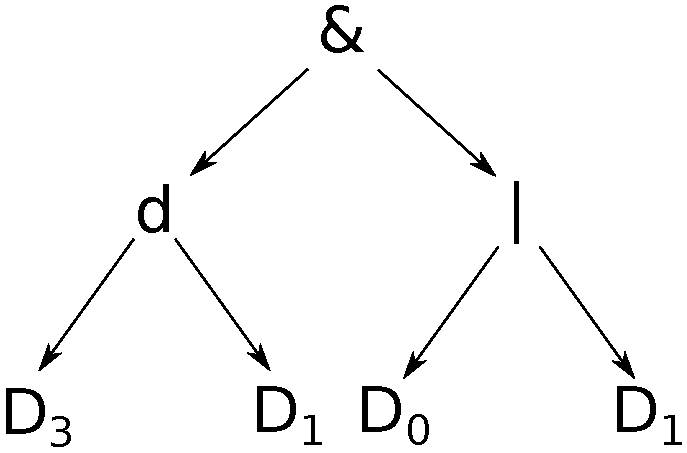
\includegraphics[width=8cm]{img/tree.pdf}
\caption{Primjer programskog isječka prikazanog binarnim stablom.}
\label{tree}
\end{figure}

Potreban je i isječak koda koji označava \emph{don't care} simbol, a koji će za svaki niz bitova koje dobije na ulazu vratiti 1.
On je prikazan na slici \ref{dnc} i označava operaciju $D_{0}D_{0}\sim|$, a preuzet je iz \citep{4}.

\begin{figure}
\centering
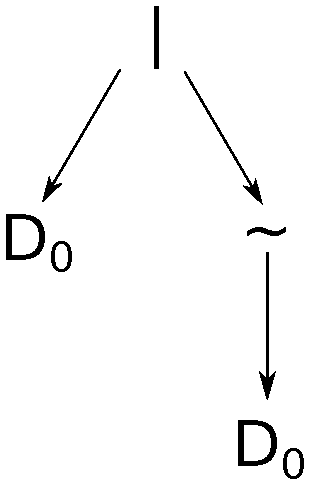
\includegraphics[height=6cm]{img/dnc.pdf}
\caption{Isječak koda korišten kao \emph{don't care} simbol.}
\label{dnc}
\end{figure}

U \emph{Explore} načinu rada, na početku od okoline dobijemo ulazni podatak \emph{s}.
U ovisnosti o \emph{s}, formira se \emph{match set} [\emph{M}].
[\emph{M}] se sastoji od svih pravila iz populacije [\emph{P}] koja odgovaraju ulazu \emph{s}.

Za pravilo \emph{cl}\footnote{Od engleskog "\emph{Classifier}"} kažemo da odgovara ulazu \emph{s}, ako svaki isječak koda za zadani ulaz \emph{s} na izlazu daje 1.

\chapter{Rezultati}


\chapter{Zaključak}


\bibliography{literatura}
\bibliographystyle{fer}

\begin{sazetak}
Sažetak na hrvatskom jeziku.

\kljucnerijeci{Ključne riječi, odvojene zarezima.}
\end{sazetak}

\engtitle{Application of LCS on Classification Problems}
\begin{abstract}
Abstract.

\keywords{Keywords.}
\end{abstract}

\end{document}

